
\section{Gaussian Mixtures}

The best discriminant between two hypotheses is the likelihood ratio.
From investigating the features we have learned that we are dealing with a multivariate dataset with complex correlations that cannot simply be described by guessing and fitting probability density functions to each feature. 

\subsection{One Dimension}

One possibility explored here is to estimate the feature distributions for signal and background in the form of Gaussian Mixture Models (GMM). 

For a simple one-dimensional case this is simply the density function is approximated by a sum of weighted, different normal distributions.
The GMM thus is given by

$$
p(x) = \sum_{i=1}^{n} w_{i}\cdot \mathcal{N}(x|\mu_i,\sigma_i)
$$
with the number of Gaussians $n$, the weights $w_i$ and the normal distributions 

$$
\mathcal{N}(x|\mu,\sigma) = \frac{1}{\sqrt{2\pi\sigma^{2}} }  \exp\left(-\frac{(x-\mu)^{2} }{2\sigma^{2}}\right)
$$

with means $\mu_i$ and standard deviations $\sigma_i$.


\subsection{Multivariate Model}


A Multivariate Gaussian Mixture Model is the extension into $d$ dimensions that uses multivariate Gaussian distributions 

$$
\mathcal{N}(x \mid \mu, \Sigma) = \frac{1}{(2\pi)^{d/2} |\Sigma|^{1/2}} \exp \left( -\frac{1}{2} (x - \mu)^\top \Sigma^{-1} (x - \mu) \right) 
$$

containing covariance matrices $\Sigma_i$ between input features $x$.


\subsection{EM-Algorithm}

The implementation of this method in sklearn uses the iterative EM algorithm to estimate the parameters of the individual Gaussians for a given dataset. This algorithm alternates between an expectation step to evaluate the model on the latest parameters, and a maximization step that updates the parameters based on the previous expectation step. Details on the exact EM-alogrithm used for Gaussian mixtures are elaborated in \href{https://scikit-learn.org/stable/modules/mixture.html#expectation-maximization}{sklearn user guide}.


\clearpage
\section{Python example}


\begin{lstlisting}[language=Python]
from sklearn.mixture import GaussianMixture

# features with unkown pdf
x_train = ... 

# parameter: number of gaussians
gmm = GaussianMixture(n_components=2) 

# EM-algorithm 
gmm.fit(x_train) 

# validation data-points from the same distribution
x_val = ... 
# log-likelihood for each sample
prob = gmm.score_samples(x_val) 
\end{lstlisting}


\section{Log-Likelihood Discriminator}

For our purpose we want to discriminate between two classes. 
We therefore generate two GMMs, one from signal training data and one from background training data. To classify a given dataset, the Log-Likelihood is calculated for both the signal $\mathcal{L}(x|s)$ and background $\mathcal{L}(x|b)$ hypothesis, and the Log-Likelihood Ratio (LLR) is calculated.

$$
LLR(x) = \log \left(\frac{\mathcal{L}(x|s)}{\mathcal{L}(x|b)}\right) = \log \mathcal{L}(x|s) - \log \mathcal{L}(x|b)
$$

To predict whether the Likelihood Ratio value of a sample is interpreted as signal or background a critical value $\lambda_{\text{crit}}$ is needed. 


\begin{align*}
LLR(x) > \lambda_{\text{crit}} \quad &\Rightarrow \quad \text{signal} \\
LLR(x) \le \lambda_{\text{crit}} \quad &\Rightarrow \quad \text{background}
\end{align*}


The explicit goal of this exercise is to reach the best AMS score. Thus, a validation dataset is used to threat the critical value as a hyperparameter. The LLRs for each sample in the validiation dataset $(x_{\text{val}},y_{\text{val}} )$ is calculated. The range of sensible critical values lies within the interval of minimum and maximum reached ratios $[LLR_{\min}(x_\text{val},\,LLR_{\max}(x_\text{val} )]$. 
The AMS score is calculated for $N_\text{stops}$ evenly spaced values in the interval and the critical value  which reaches the best score is chosen for further use. 



\subsection{Implementation}

The training data is split into $75\,\%$ for training and $15\,\%$ fr validation purposes.


The more features, the larger the computational effort. Thus the number of features was reduced with a Principal Component Analysis (PCA). This is an unsupervised method that reduces the dimensionality of a dataset and minimizes correlation between the so-called "principal components" while trying to maintain as much variance as possible, see figure \ref{fig:pca-evr}. A disadvantage is that the principal components are not physically interpretable. One benefit for the use with this classification method is that the principal components generated with this method visually resemble linear combinations of normal distributions, see figure \ref{fig:hists-pca}. 

The more components are generated, the more variance in the original data can be maintained.

\begin{figure}
    \centering
    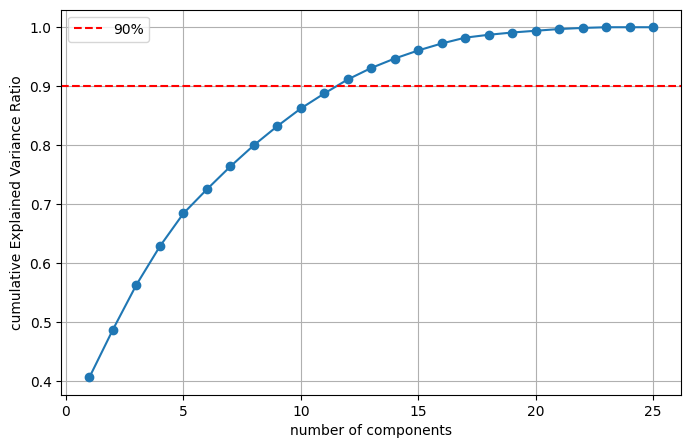
\includegraphics[width=0.8\textwidth]{img/Pasted image 20240805114251.png}
    \caption{PCA: Explained Variance Ratio retained, depending on the number of components.}
    \label{fig:pca-evr}
\end{figure}

Manual tests found that the use of only 8 components for the PCA, while only capturing $80\,\%$ of original variance, found good AMS scores. 



\begin{figure}
    \centering
    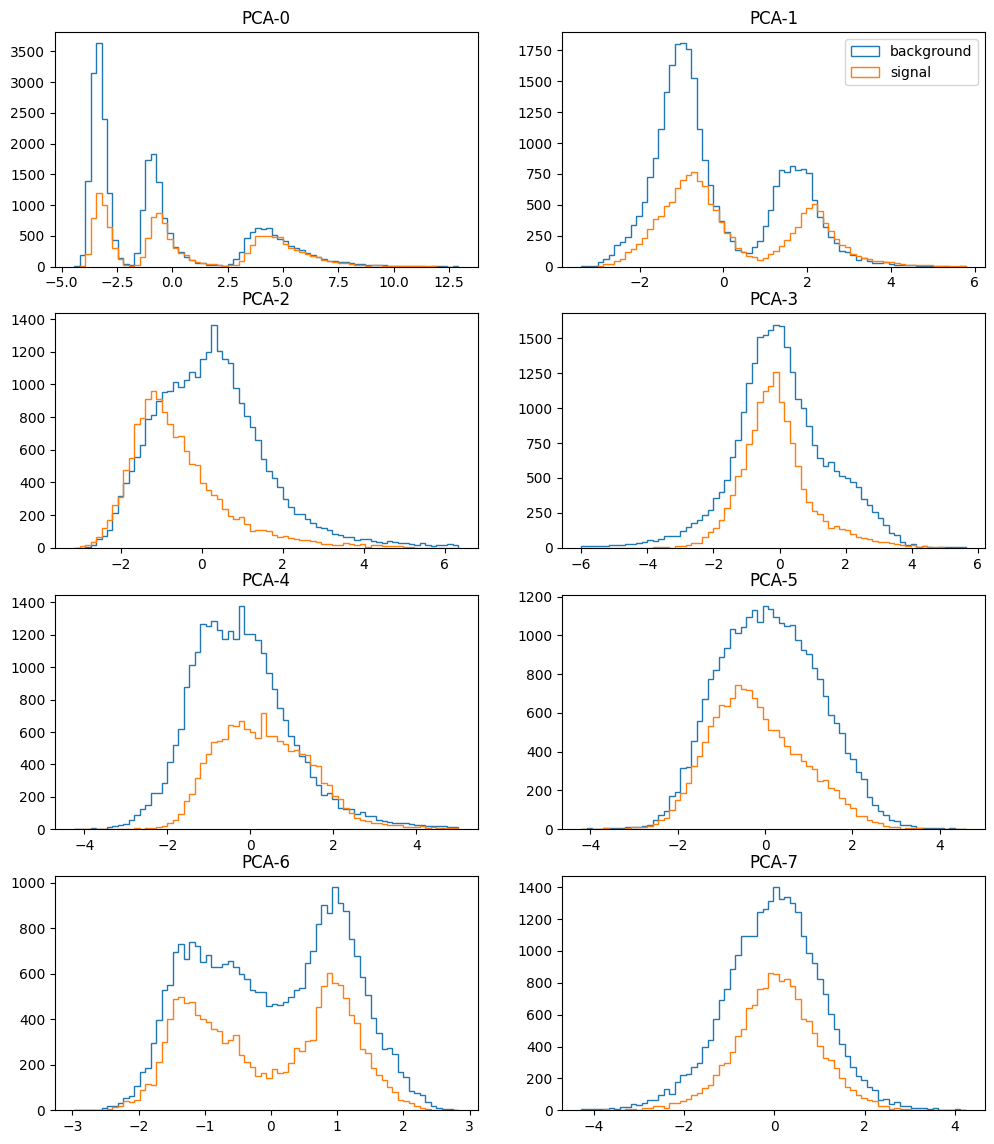
\includegraphics[width=0.9\textwidth]{img/Pasted image 20240805115045.png}
    \caption{Histograms of the principle components for signal (orange) and background (blue) for the training dataset.}
    \label{fig:hists-pca}
\end{figure}


\begin{figure}
    \centering
    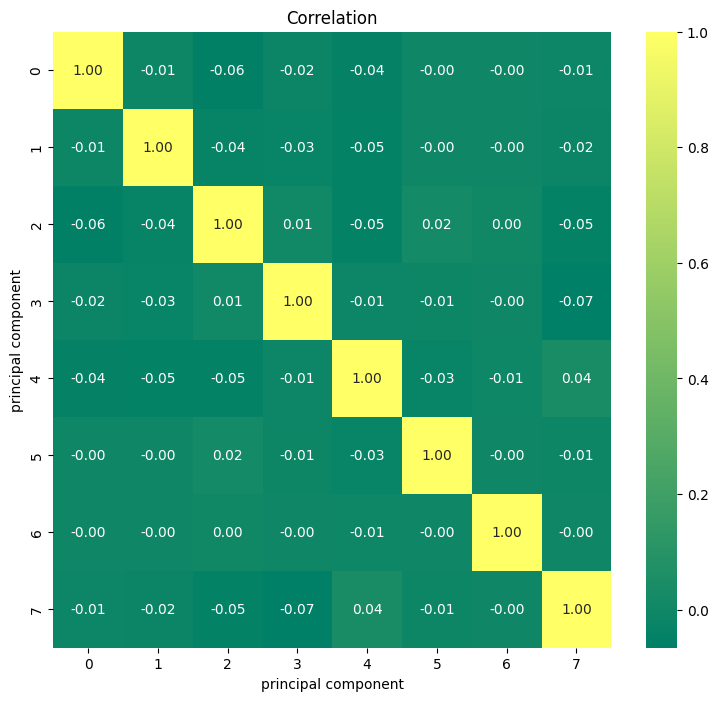
\includegraphics[width=0.65\textwidth]{img/Pasted image 20240805120402.png}
    \caption{Correlation matrix after the PCA.}
    \label{fig:corrmatrix}
\end{figure}


\begin{figure}
    \centering
    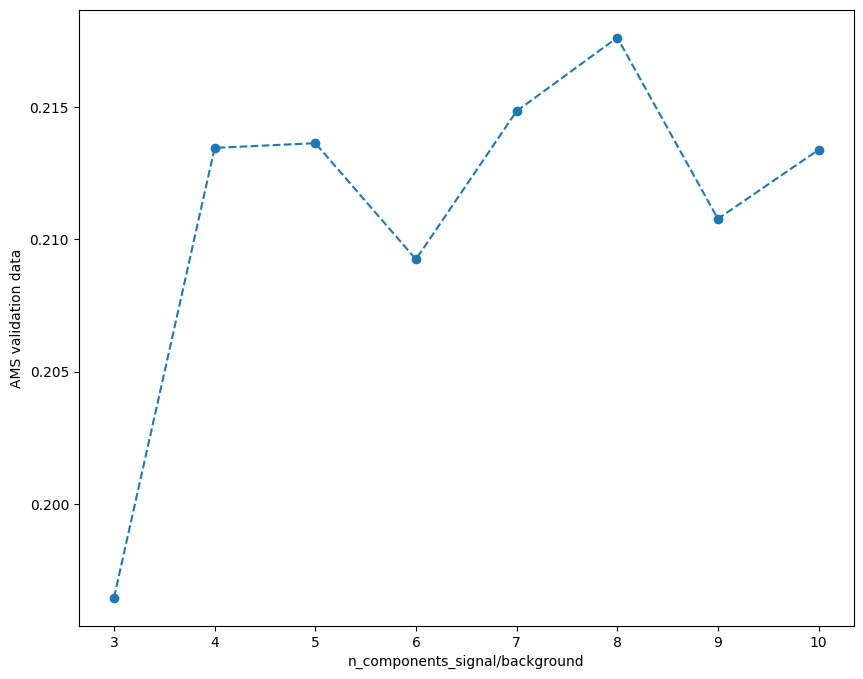
\includegraphics[width=0.65\textwidth]{img/Pasted image 20240805120618.png}
    \caption{Search for the optimal number of Normal distributions used in the Gaussian Mixtures.}
    \label{fig:n-search}
\end{figure}


Other hyperparameters that influence the AMS score are the number of Gaussians $n$ used to approximate the mutivarariate distributions of signal and background. The same value $n$ is used for both classes. A hyperparameter search suggests the use of $n=8$, see figure \ref{fig:n-search}. This search utilized $5$ different initializations and warm starts that utilized solutions of previous iterations. However, for individual seeds, other values also achieved good results. 



Besides the multivarariate \texttt{GaussianMixture}, another sklearn class \texttt{BayesianGaussianMixture} was tested and reached on average slightly more consistent results. Details on the differences due to its Bayesian nature can be found in the  \href{https://scikit-learn.org/stable/modules/mixture.html#variational-bayesian-gaussian-mixture}{sklearn user guide}, the practical usage however remains the same. 

The maximum AMS score reached with the \texttt{atlas-higgs-challenge-2014-v2\_part.root} dataset in the explained configuration is $0.498$. 
A test of the full \texttt{atlas-higgs-challenge-2014-v2.root} dataset found a score of $1.71$. However, it should be mentioned that (due to computational times) only one iteration was used to find the GMMs for signal and background each. 


\begin{figure}
    \centering
    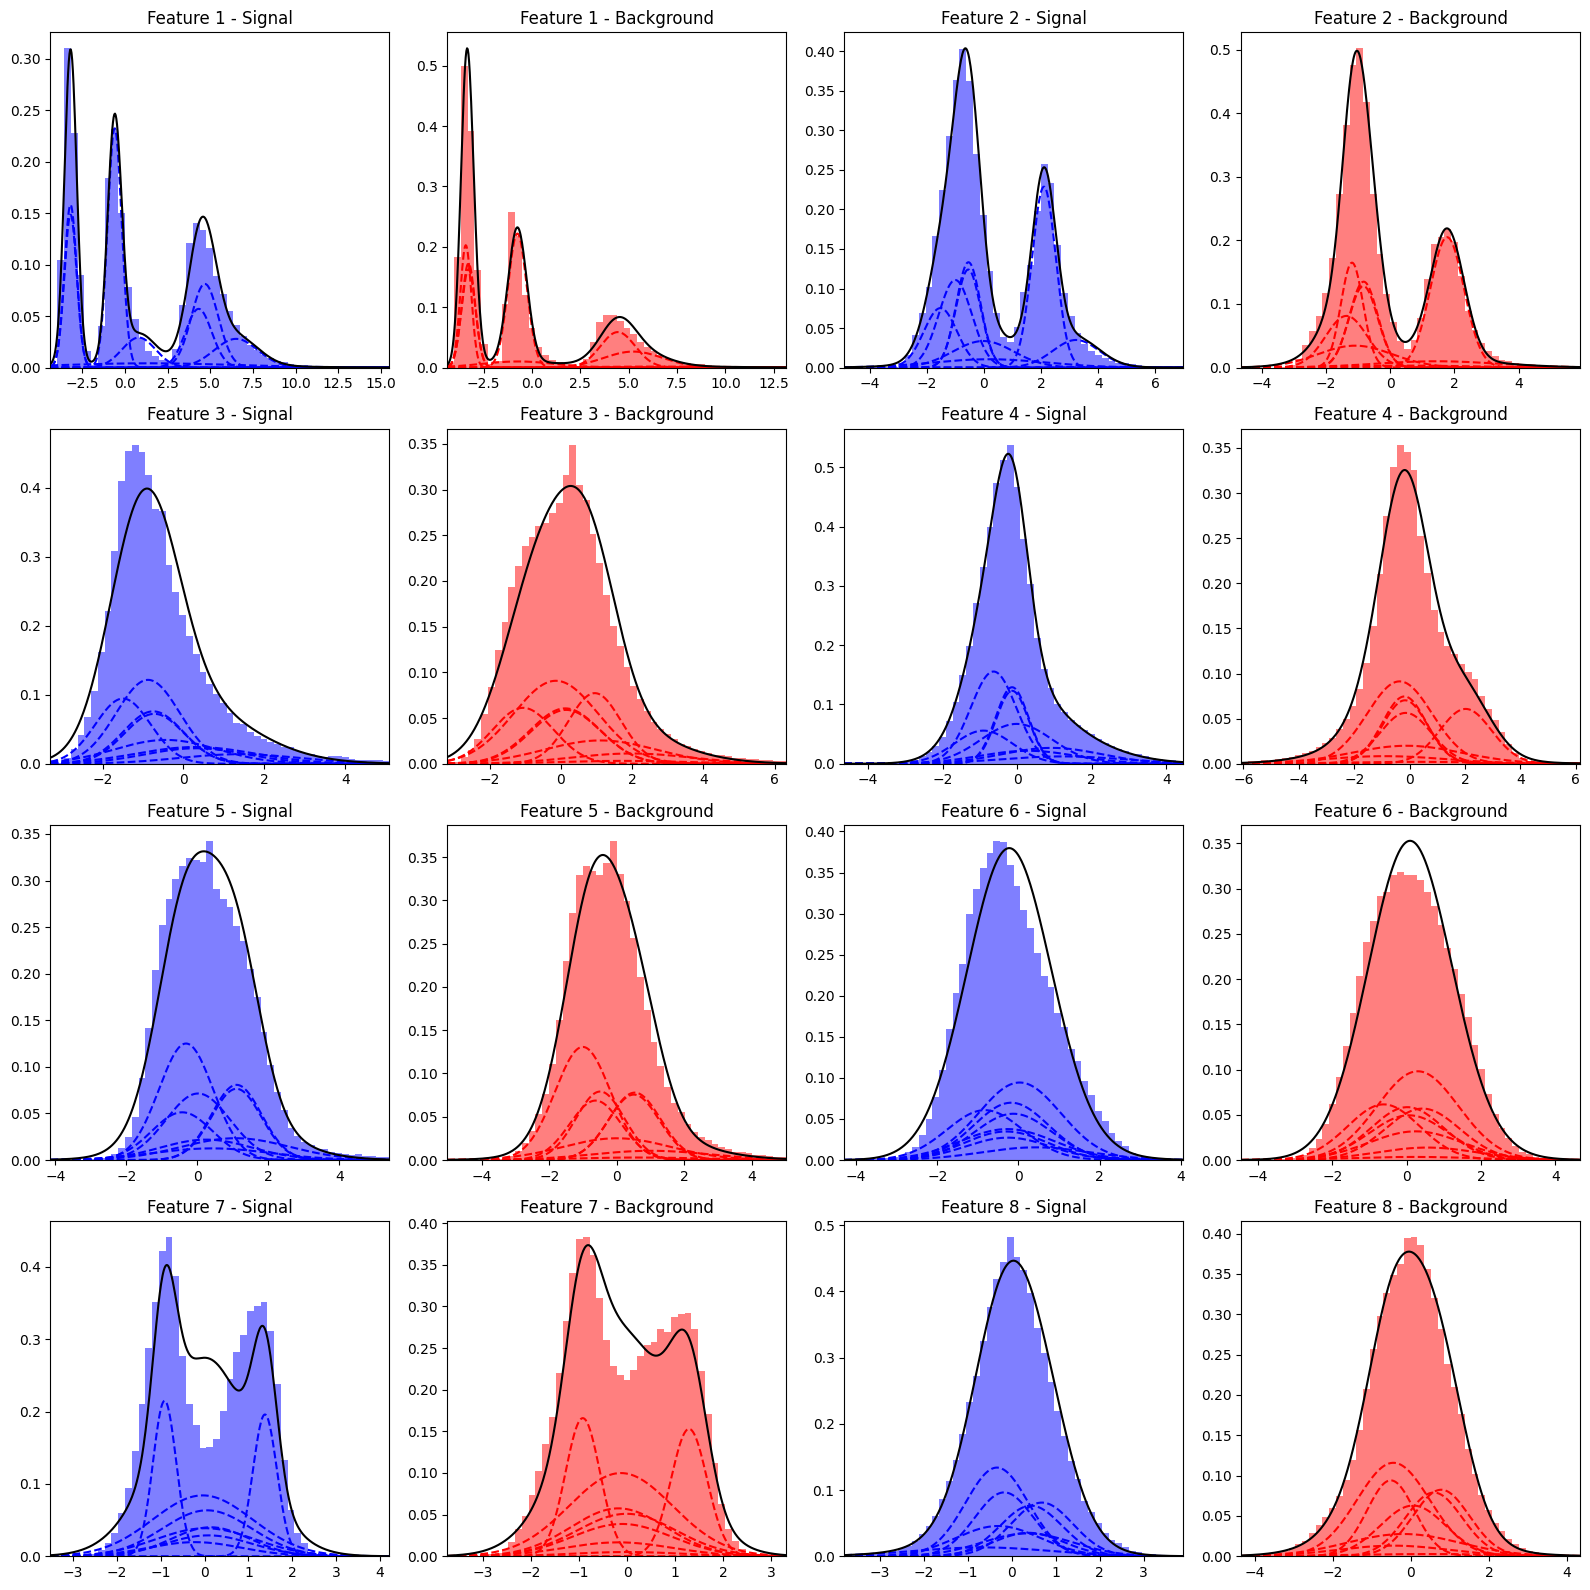
\includegraphics[width=\textwidth]{img/fullmodel.png}
    \caption{Bayesian GMM: Signal and background histograms and the GMMs found from the training data. Dotted lines represent the individual, weighted normal distributions that sum up to the complete functions (black).}
    \label{fig:bgmm-plot}
\end{figure}

Figure \ref{fig:bgmm-plot} shows the distributions of the training signal and background data and the GMM used for each feature individually. Visually one can observe how feature 1, 2, 4 and 8 are well described. However, especially feature 7 seems to be badly approximated by the Mixture Model. Different methods for initializing the weighs, means and covariances of the Gaussians we're tested.
Sklearn allows to specify whether these parameters are chosen by k-means, k-means++, random initializations, or by randomly selected data-points. From these methods k-means++ was found to reach the best results. 
There is also the possibility to pass pre-specified initial means, weights and precisions to the \texttt{GaussianMixture} class. Estimating reasonable values by hand however did not improve the results. 


To fix this deviation, another implementation was tested, that would find an optimal GMM for each input-feature independently. The drawback is that this method does neglect correlations between the features. So, while the histograms of the training features are described very accurately, the best AMS score reached for the partial dataset is $0.24$, the complete training dataset finds an AMS score of $0.80$.



\begin{figure}
    \centering
    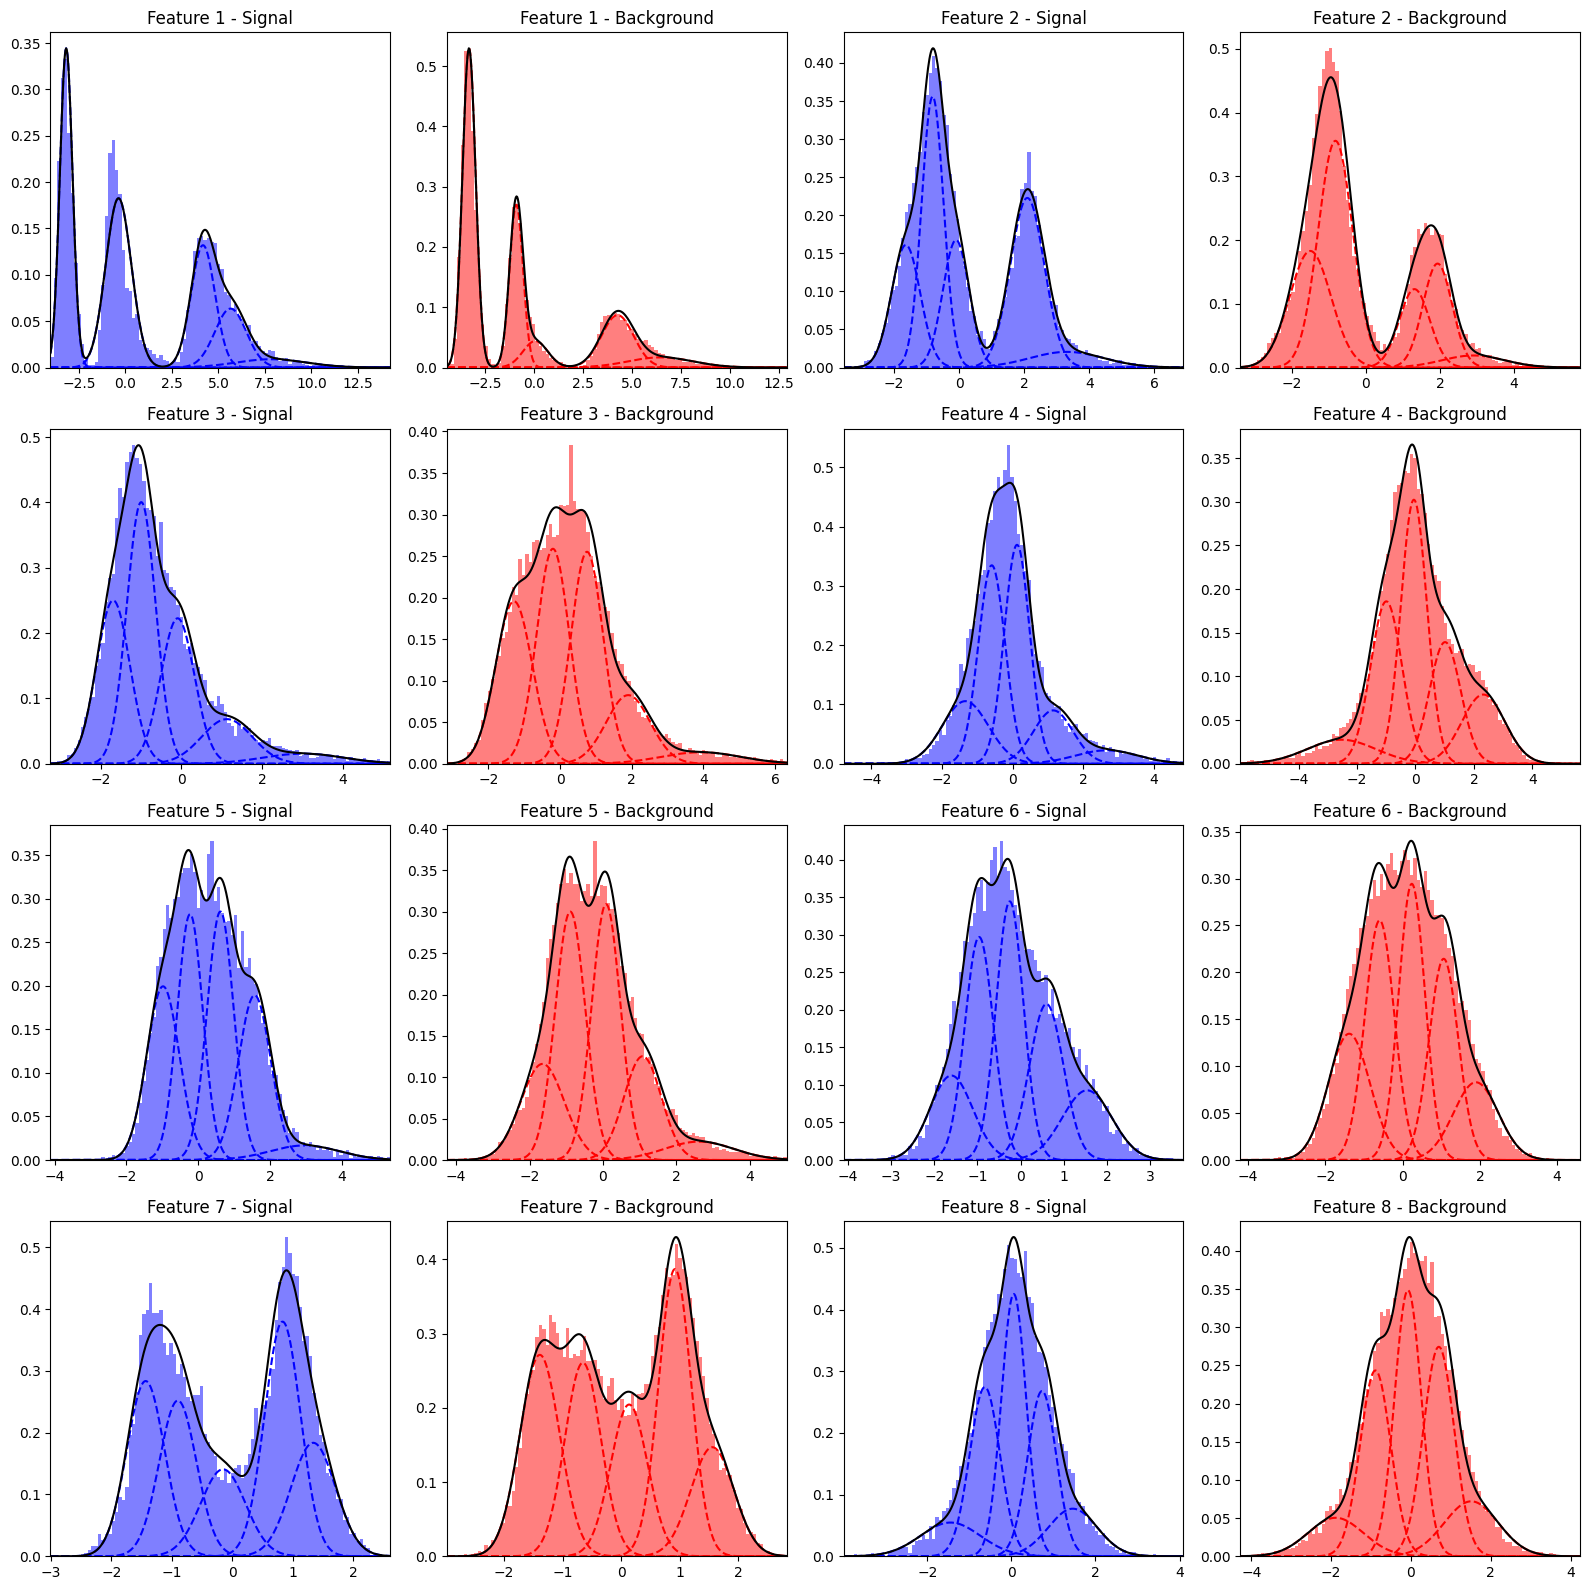
\includegraphics[width=\textwidth]{img/tightfit.png}
    \caption{Uncorrelated GMMs: Signal and background histograms and the Gaussians found from the training data.}
    \label{fig:enter-label}
\end{figure}



\clearpage
%%%%%%%%%%%%%%%%%%%%%%%%%%%


\appendix

\section{Appendix}


This is example code on how to use the explained classifier:

\begin{lstlisting}[language=Python]
clf = BGMClassifier(n_components_signal=8, n_components_background=8)
clf.train(x_train=x_train, y_train=y_train)

crit_val = bgmclf.findCriticalValue(x_val, y_val, w_val, scorer_function=ams_wrapper, num_points=100)

predictions = bgmclf.predict(x_test)

print(ams_wrapper(predictions, y_test, w_test))
\end{lstlisting}


What follows is the code for the Bayesian Gaussian Mixture classifier class:

\begin{lstlisting}[language=Python]

class BGMClassifier:
    def __init__(self, n_components_signal=5, n_components_background=5):
        self.n_components_signal = n_components_signal
        self.n_components_background = n_components_background
    
    def train(self, x_train, y_train):
        """
        Trains two Bayesian GMMs for signal and background data.

        Parameters:
        - x_train: array-like of shape (n_samples, n_features)
            The input samples.
        - y_train: array-like of shape (n_samples,)
            The target values (binary labels: 0 for background, 1 for signal).
        - sample_weight: array-like of shape (n_samples,), optional
            The sample weights for training.
        """
        
        # separate signal and background
        self.signal_data = x_train[y_train.astype(bool)]
        self.background_data = x_train[~y_train.astype(bool)]
        

        # initialize and fit
        self.signal_bgm = BayesianGaussianMixture(n_components=self.n_components_signal, n_init=5, init_params='k-means++', random_state=None, max_iter=1000, tol=5e-4, warm_start=True)
        self.background_bgm = BayesianGaussianMixture(n_components=self.n_components_background, n_init=5, init_params='k-means++', random_state=None, max_iter=1000, tol=5e-4, warm_start=True)
        #init_params='random_from_data', 
        
        self.signal_bgm.fit(self.signal_data)
        print('Signal BGM calculated!')
        self.background_bgm.fit(self.background_data)
        print('Background BGM calculated!')

    
    def calculateLLR(self, x):
        """
        Calculate the log-likelihood ratios for the signal and background hypotheses.

        Parameters:
        - x: numpy array of shape (n_samples, n_features)

        Returns:
        - log_likelihood_ratio: numpy array of log-likelihood ratios
        """
        
        log_likelihood_signal = self.signal_bgm.score_samples(x)
        print('Signal Likelihood calculated!')
        log_likelihood_background = self.background_bgm.score_samples(x)
        print('Background Likelihood calculated!')

        log_likelihood_ratio = log_likelihood_signal - log_likelihood_background
        return log_likelihood_ratio

    
    def predict(self, x):
        """
        Predict the class labels (signal or background) for the given input data.

        Parameters:
        - x: numpy array of shape (n_samples, n_features), input data

        Returns:
        - probs: numpy array of predicted labels (0 for background, 1 for signal)
        """
        
        llr = self.calculateLLR(x)
        probs = np.zeros_like(llr)
        probs[llr > self.critical_value] = 1
        return probs
        

    def findCriticalValue(self, x_val, y_val, w_val, scorer_function, num_points=100):
        """
        Find the best critical value for the log-likelihood ratio using validation data.

        Parameters:
        - x_val: numpy array of shape (n_samples, n_features), validation data
        - y_val: numpy array of boolean values, true labels for validation data
        - w_val: numpy array of weights
        - scorer_function: function that evaluates the performance (ams_scorer)
        - num_points: number of points to evaluate for finding the critical value

        Returns:
        - best_critical_value: the critical value that maximizes the scorer function
        """
        
        llr = self.calculateLLR(x_val)

        min_llr, max_llr = np.min(llr), np.max(llr)
        thresholds = np.linspace(min_llr, max_llr, num_points)

        best_score = -np.inf
        best_critical_value = None
        for threshold in thresholds:
            y_pred = llr > threshold
            score = scorer_function(y_pred, y_val, w_val)

            if score > best_score:
                best_score = score
                best_critical_value = threshold

        print(f'Best critical value {best_critical_value} for validation score: {best_score}')

        # store the criticial value for later classifcation use
        self.critical_value = best_critical_value
        return best_critical_value, best_score

    def plotDistributions(self):
        """
        Plots the histograms of training signal and background data along with the fitted
        Bayesian Gaussian Mixture distributions for each feature. Signal plots
        are on the left, background plots are on the right.
        """
        
        ...

\end{lstlisting}


